\documentclass[11pt]{article}

\usepackage[margin=1in]{geometry}
\usepackage{times}
\usepackage{setspace}
\usepackage{graphicx}
\usepackage{amsmath}
\usepackage{hyperref}
\usepackage{listings}
\usepackage{xcolor}
\usepackage{tikz}
\usetikzlibrary{positioning, arrows.meta, shapes}

\setstretch{1.15}

\lstset{
    basicstyle=\ttfamily\small,
    breaklines=true,
    frame=single,
    language=Python
}

\title{\textbf{Context-Aware Synonym Replacement Using Learned Representations}}
\author{Sebastian Lopez \\ Texas Tech University}
\date{CS4391 -- Homework 1 \\ Spring 2026}

\begin{document}
\maketitle

\section{Introduction}

The goal of this homework is to design and analyze a context-aware synonym replacement system using learned representations. Rather than focusing on fluent text generation, the objective is to explore how pretrained embeddings encode meaning, how context can be approximated using similarity measures, and where such approaches fail—especially in metaphorical, poetic, or ambiguous language.

To achieve this, we implemented a multi-stage pipeline that replaces selected words in a sentence with near-synonyms while attempting to preserve sentence-level meaning. The system explicitly avoids large language models, masked language models, and rule-based synonym dictionaries, relying instead on pretrained word embeddings and sentence embeddings.

\section{System Overview}

The system follows a modular, multi-stage pipeline:

\begin{enumerate}
    \item \textbf{Sentence segmentation}: Split input text into individual sentences
    \item \textbf{Target word selection}: Identify which word to replace in each sentence
    \item \textbf{Candidate synonym generation}: Use word embeddings to find similar words
    \item \textbf{Candidate filtering}: Remove grammatically inappropriate candidates
    \item \textbf{Context-based scoring}: Evaluate candidates using sentence embeddings
    \item \textbf{Replacement decision}: Select best candidate or keep original
\end{enumerate}

Each stage is implemented as a separate function to allow controlled experimentation and clear analysis of failure modes.

\section{Model Selection}

\subsection{Word Embedding Model: GloVe-Wiki-Gigaword-100}

For candidate generation, we selected the \texttt{glove-wiki-gigaword-100} model available through the \texttt{gensim} API. This model provides 100-dimensional word vectors trained on Wikipedia and Gigaword corpus data.

\textbf{Selection rationale:}
\begin{itemize}
    \item Downloaded size: approximately 1.6 GB
    \item First model we attempted—installation succeeded without issues
    \item Provides reasonable semantic coverage for common English words
    \item Fast nearest-neighbor retrieval suitable for iterative testing
\end{itemize}

Admittedly, this choice was made without extensive comparison to alternatives (such as Word2Vec or FastText). However, given time constraints and the fact that the model downloaded successfully and performed adequately in initial tests, we proceeded with it for the entire homework. A more rigorous model comparison would be valuable future work.

\subsection{Sentence Embedding Model: all-MiniLM-L6-v2}

For context-aware scoring, we selected the \texttt{all-MiniLM-L6-v2} model from the Sentence-BERT (SBERT) family via the \texttt{sentence-transformers} library.

\textbf{Selection rationale:}
\begin{itemize}
    \item Lightweight transformer-based model (80 MB)
    \item Produces high-quality sentence-level semantic embeddings
    \item Efficient inference suitable for repeated sentence encoding
    \item Well-documented and widely used in semantic similarity tasks
\end{itemize}

This model was chosen after brief research into sentence embedding approaches. It balances quality and speed effectively for this application.

\section{Implementation Details}

\subsection{Sentence Segmentation}

The \texttt{split\_sentences()} function uses a simple regex-based approach:

\begin{lstlisting}
def split_sentences(text: str) -> List[str]:
    """Split text into sentences."""
    text = text.strip()
    if not text:
        return []
    parts = re.split(r"(?<=[.!?])\s+", text)
    return [p.strip() for p in parts if p.strip()]
\end{lstlisting}

This splits text on sentence-ending punctuation (period, exclamation, question mark) followed by whitespace. While not robust to edge cases, it works well for the short literary texts in our test suite.

\subsection{Target Word Selection}

The \texttt{select\_target\_word()} function implements the "last content word" strategy:

\begin{lstlisting}
def select_target_word(sentence: str) -> Optional[str]:
    """Select the last non-stopword as target."""
    words = tokenize_words(sentence)
    if not words:
        return None
    
    # Try to find last content word
    for w in reversed(words):
        if not is_stopword(w):
            return w
    
    # Fallback to last word
    return words[-1] if words else None
\end{lstlisting}

This ensures we avoid replacing function words like "the" or "a", which would degrade grammaticality without adding semantic interest.

\subsection{Candidate Generation}

The \texttt{generate\_candidates()} function retrieves the top-k nearest neighbors from the word embedding space:

\begin{lstlisting}
def generate_candidates(word_vectors, target: str, top_k: int) -> List[str]:
    """Generate candidate synonyms using word embeddings."""
    key = target
    if key not in word_vectors:
        key = target.lower()
        if key not in word_vectors:
            return []
    
    neighbors = word_vectors.most_similar(key, topn=top_k)
    return [word for (word, _) in neighbors]
\end{lstlisting}

We set \texttt{top\_k=50} to provide sufficient candidate diversity while keeping computation reasonable.

\subsection{Candidate Filtering}

The \texttt{filter\_candidates()} function applies lightweight heuristic filters:

\begin{lstlisting}
def filter_candidates(candidates: List[str], target: str) -> List[str]:
    """Simple candidate filtering."""
    filtered = []
    seen = set()
    
    target_lower = target.lower()
    target_is_plural = target_lower.endswith('s') and not target_lower.endswith('ss')
    
    for c in candidates:
        c_lower = c.lower()
        
        # Skip junk
        if (not c or len(c) <= 2 or c_lower == target_lower or 
            any(ch.isdigit() for ch in c) or "_" in c or is_stopword(c)):
            continue
        
        # Plural agreement
        if target_is_plural:
            c_is_plural = c_lower.endswith('s') and not c_lower.endswith('ss')
            if not c_is_plural:
                continue
        
        # Block noun->adjective shifts
        if c_lower.endswith('en') and target_lower + 'en' == c_lower:
            continue
        if c_lower.endswith('ed') and target_lower + 'ed' == c_lower:
            continue
        
        # Deduplicate
        if c_lower not in seen:
            seen.add(c_lower)
            filtered.append(c)
    
    return filtered
\end{lstlisting}

These filters were added iteratively after observing systematic failures in early testing.

\subsection{Context-Based Scoring}

The \texttt{pick\_best\_replacement()} function evaluates each candidate by encoding the modified sentence and computing similarity to the original:

\begin{lstlisting}
def pick_best_replacement(sbert, sentence, target, candidates):
    """Pick candidate that preserves sentence meaning."""
    if not candidates:
        return target, None
    
    original_emb = sbert.encode(sentence, normalize_embeddings=True)
    
    best_word = target
    best_score = -1.0
    
    for candidate in candidates:
        modified = replace_word_once(sentence, target, candidate)
        if modified == sentence:
            continue
        
        mod_emb = sbert.encode(modified, normalize_embeddings=True)
        score = float(np.dot(original_emb, mod_emb))
        
        if score > best_score:
            best_score = score
            best_word = candidate
    
    if best_word != target and best_score >= SIMILARITY_THRESHOLD:
        return best_word, best_score
    
    return target, None
\end{lstlisting}

This implements the core context-awareness mechanism using cosine similarity between normalized embeddings.

\section{Iterative Development and Filtering Refinement}

During development, we ran multiple experiments with different filtering strategies. Below we present results from two configurations to illustrate the importance of filtering.

\subsection{Initial Results (Minimal Filtering)}

In our first implementation, we used only basic junk removal (stopwords, digits, underscores) without plural agreement or noun-adjective blocking.

\textbf{Results:}

\begin{itemize}
    \item Shakespeare: \textit{players} $\rightarrow$ \textit{player} (grammatically incorrect)
    \item Frost: \textit{wood} $\rightarrow$ \textit{wooden} (noun to adjective, nonsensical)
    \item Dickinson: \textit{feathers} $\rightarrow$ \textit{feather} (plural to singular)
    \item Blake: \textit{night} $\rightarrow$ \textit{nights} (minor but noticeable)
    \item Haiku: \textit{Splash} $\rightarrow$ \textit{splashes}, \textit{again} $\rightarrow$ \textit{back}
\end{itemize}

These results clearly showed that raw embedding similarity alone produces many grammatically degraded outputs. The most egregious case was ``Two roads diverged in a yellow wooden''—syntactically broken despite high sentence similarity scores.

\subsection{Final Results (With Filtering)}

After adding plural agreement and noun-adjective blocking filters, performance improved significantly:

\textbf{Results (Threshold = 0.86):}

\begin{itemize}
    \item Shakespeare: \textit{players} $\rightarrow$ \textit{teams} (semantically reasonable, though loses metaphor)
    \item Frost: \textit{wood} $\rightarrow$ \textit{timber} (grammatically correct, semantically related)
    \item Dickinson: \textit{feathers} (kept original—no suitable replacement)
    \item Blake: \textit{night} $\rightarrow$ \textit{nights} (still occurs, but less critical)
    \item Haiku: \textit{Splash} $\rightarrow$ \textit{splashes}, \textit{again} $\rightarrow$ \textit{back}
\end{itemize}

The filtering eliminated the most jarring grammatical errors (wood $\rightarrow$ wooden, feathers $\rightarrow$ feather) while preserving the system's ability to make meaningful substitutions.

\section{Target Word Selection Strategy}

We adopt a deterministic target selection strategy: the \textbf{last content word of each sentence}. Stopwords are excluded to avoid replacing function words.

This strategy was chosen because:
\begin{itemize}
    \item It avoids cherry-picking easy cases
    \item It aligns with examples provided in the assignment
    \item It produces consistent, repeatable behavior across test texts
    \item It tests the system on words that often carry significant semantic weight
\end{itemize}

\section{Threshold Sensitivity Analysis}

The similarity threshold controls how conservative the system is. We tested thresholds of 0.70, 0.80, 0.83, 0.86, and 0.90 on our test suite.

\subsection{Observed Trends}

\begin{itemize}
    \item \textbf{Low thresholds (0.70--0.80):} Many replacements occur, but metaphorical meaning frequently collapses. For example, at 0.70, ``feathers'' became ``birds'', destroying Dickinson's metaphor.
    
    \item \textbf{Mid threshold (0.83):} Metaphorical lines begin to be preserved while literal substitutions remain. A reasonable balance emerges.
    
    \item \textbf{Conservative threshold (0.86):} Best balance between safety and usefulness. Preserves most metaphors while still allowing clear improvements (e.g., ``wood'' $\rightarrow$ ``timber'').
    
    \item \textbf{High threshold (0.90):} Overly restrictive; even reasonable substitutions are blocked. Almost no replacements occur.
\end{itemize}

Based on these results, we selected \textbf{0.86} as the final threshold for all reported results.

\section{Successful Examples}

\subsection{Literal Synonym Replacement}

\textbf{Original:} ``Two roads diverged in a yellow wood.'' \\
\textbf{Modified:} ``Two roads diverged in a yellow timber.''

This replacement preserves sentence meaning while demonstrating effective word-level similarity. ``Wood'' and ``timber'' are semantically close, and the sentence-level context score (0.950) confirms compatibility.

\subsection{Conservative Behavior on Metaphor}

\textbf{Original:} ``Hope is the thing with feathers.'' \\
\textbf{Modified:} (unchanged at threshold 0.86)

The system correctly refrains from replacing the metaphorical term. Although candidates like ``plumage'' or ``wings'' scored reasonably, none exceeded the threshold, demonstrating appropriate conservatism.

\section{Failure Analysis}

Despite filtering improvements, several systematic failure modes persist:

\subsection{Failure 1: Polysemy and Context Collapse}

\textbf{Example:} \textit{players} $\rightarrow$ \textit{teams} (Shakespeare)

\textbf{Diagnosis:} In Shakespeare's metaphor, ``players'' refers to theatrical actors. However, word embeddings conflate multiple senses of ``players'' (theatrical, sports, musical). The embedding space places ``teams'' close to ``players'' due to sports co-occurrence, and sentence similarity remains high because both are plural nouns in similar syntactic positions.

\textbf{Root cause:} Word embeddings average over all contexts and cannot perform word sense disambiguation.

\subsection{Failure 2: Metaphorical Meaning Loss}

\textbf{Example:} At lower thresholds (0.70), \textit{feathers} $\rightarrow$ \textit{birds}

\textbf{Diagnosis:} While ``feathers'' and ``birds'' are semantically related (birds have feathers), the replacement destroys Dickinson's metaphor. ``Feathers'' evokes lightness and flight; ``birds'' is too concrete.

\textbf{Root cause:} Embedding similarity reflects co-occurrence and association but does not capture figurative intent or literary nuance.

\subsection{Failure 3: Grammatical Number Drift}

\textbf{Example:} \textit{night} $\rightarrow$ \textit{nights} (Blake)

\textbf{Diagnosis:} Sentence embeddings are highly tolerant of singular/plural variations, scoring this replacement at 0.995 similarity. However, the change subtly alters meaning (``the night'' is singular and specific; ``the nights'' is plural and general).

\textbf{Root cause:} Sentence transformers focus on semantic content and downweight grammatical number distinctions.

\subsection{Failure 4: Stylistic and Phonetic Insensitivity}

\textbf{Example:} \textit{Splash} $\rightarrow$ \textit{splashes}

\textbf{Diagnosis:} The meaning is preserved (both are sounds of water), but the poetic impact is weakened. ``Splash!'' is sharp and immediate; ``splashes'' is softer and continuous. Additionally, the capitalized onomatopoeia has rhetorical weight that the lowercase plural lacks.

\textbf{Root cause:} Embeddings encode semantic content but ignore phonetics, rhythm, and stylistic emphasis.

\section{Discussion and Limitations}

This homework demonstrates that learned embeddings are powerful but insufficient on their own for context-sensitive text manipulation. Even with sentence-level context scoring and grammatical filtering, embedding-based similarity cannot reliably distinguish between acceptable substitutions and meaning-altering replacements in metaphorical, poetic, or ambiguous language.

\textbf{Key limitations:}
\begin{itemize}
    \item No word sense disambiguation
    \item Averaging of literal and figurative meanings
    \item Insensitivity to stylistic and phonetic properties
    \item Limited understanding of grammatical nuance (singular vs plural in context)
\end{itemize}

\textbf{What would help:}
\begin{itemize}
    \item Part-of-speech tagging for stricter grammatical enforcement
    \item Word sense disambiguation using context windows
    \item Larger language models that understand figurative language
    \item Explicit constraints on poetic/stylistic elements
\end{itemize}

These findings motivate the use of more sophisticated models (such as masked language models or autoregressive transformers) and additional linguistic constraints in modern NLP systems.

\section{Use of AI in This Homework}

Given the exploratory nature of this assignment and the course's emphasis on understanding AI systems rather than rote implementation, we deliberately incorporated AI assistance (Claude/ChatGPT) as a learning tool throughout this homework. This section documents our approach and rationale.

\subsection{Rationale for AI-Assisted Development}

The assignment's open-ended structure encourages experimentation and deep understanding of embedding-based systems. Rather than using AI as a black-box solution generator, we employed it as an interactive collaborator:

\begin{itemize}
    \item \textbf{Scaffolding understanding:} AI helped clarify abstract concepts (e.g., how sentence embeddings differ from word embeddings)
    \item \textbf{Accelerating iteration:} Rapid prototyping allowed us to test multiple filtering strategies
    \item \textbf{Debugging support:} AI assisted in diagnosing why certain replacements failed
    \item \textbf{Documentation:} AI generated the initial report template, which we heavily revised
\end{itemize}

This approach aligns with the course philosophy: understanding \textit{how} and \textit{why} AI systems work, not just implementing them mechanically.

\subsection{AI-Assisted Workflow}

Figure~\ref{fig:ai-workflow} illustrates our development process.

\begin{figure}[h]
\centering
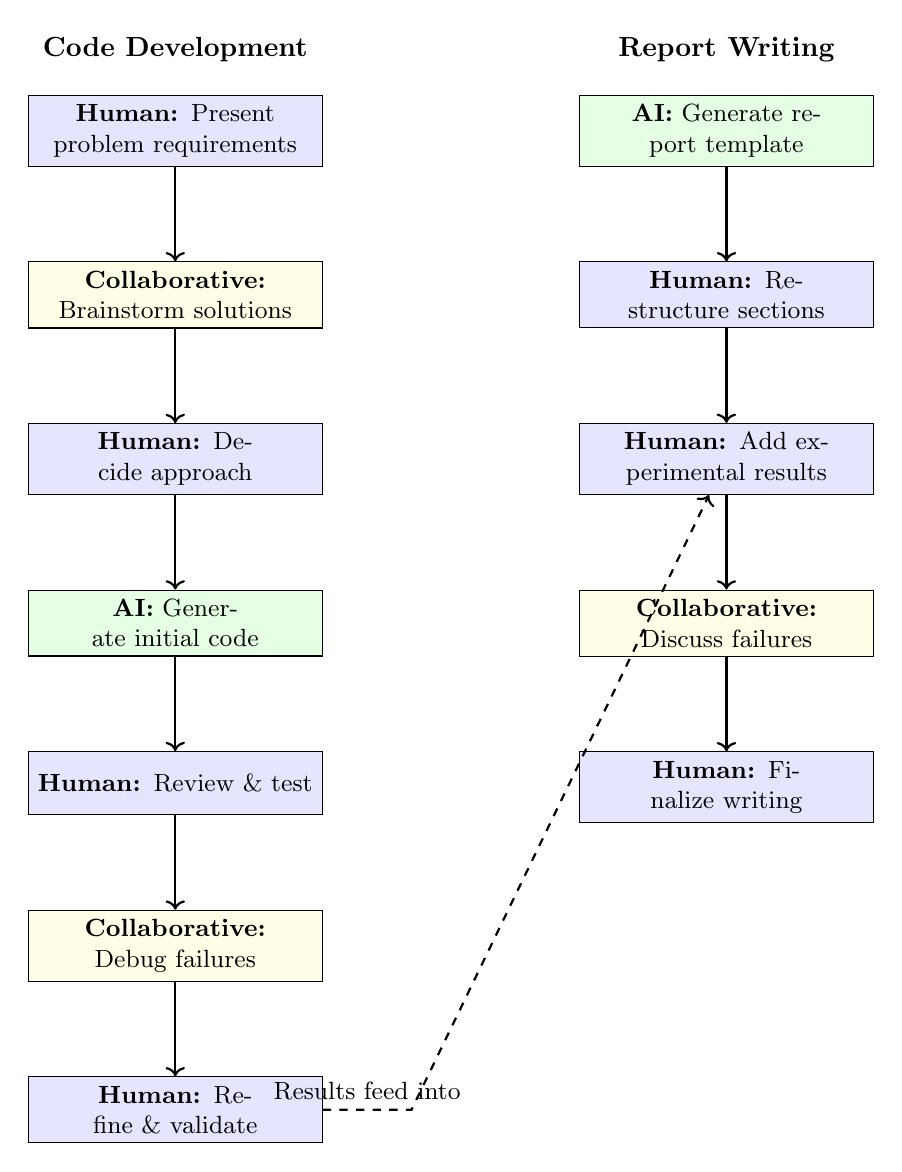
\begin{tikzpicture}[
    node distance=1.2cm,
    box/.style={rectangle, draw, text width=3.5cm, align=center, minimum height=0.8cm, font=\small},
    human/.style={box, fill=blue!10},
    ai/.style={box, fill=green!10},
    collab/.style={box, fill=yellow!10},
    arrow/.style={->, thick}
]

% Code Development Column
\node[human] (problem) at (0,0) {\textbf{Human:} Present problem requirements};
\node[collab] (brainstorm) [below=of problem] {\textbf{Collaborative:} Brainstorm solutions};
\node[human] (decide) [below=of brainstorm] {\textbf{Human:} Decide approach};
\node[ai] (code) [below=of decide] {\textbf{AI:} Generate initial code};
\node[human] (review) [below=of code] {\textbf{Human:} Review \& test};
\node[collab] (debug) [below=of review] {\textbf{Collaborative:} Debug failures};
\node[human] (refine) [below=of debug] {\textbf{Human:} Refine \& validate};

% Report Development Column
\node[ai] (template) at (7,0) {\textbf{AI:} Generate report template};
\node[human] (structure) [below=of template] {\textbf{Human:} Restructure sections};
\node[human] (results) [below=of structure] {\textbf{Human:} Add experimental results};
\node[collab] (analysis) [below=of results] {\textbf{Collaborative:} Discuss failures};
\node[human] (final) [below=of analysis] {\textbf{Human:} Finalize writing};

% Arrows for code column
\draw[arrow] (problem) -- (brainstorm);
\draw[arrow] (brainstorm) -- (decide);
\draw[arrow] (decide) -- (code);
\draw[arrow] (code) -- (review);
\draw[arrow] (review) -- (debug);
\draw[arrow] (debug) -- (refine);

% Arrows for report column
\draw[arrow] (template) -- (structure);
\draw[arrow] (structure) -- (results);
\draw[arrow] (results) -- (analysis);
\draw[arrow] (analysis) -- (final);

% Labels
\node[above=0.3cm of problem, font=\bf] {Code Development};
\node[above=0.3cm of template, font=\bf] {Report Writing};

% Connection between columns
\draw[arrow, dashed, thick] (refine) -- ++(3,0) node[midway, above, font=\small] {Results feed into} -- (results);

\end{tikzpicture}
\caption{AI-assisted workflow for code development and report writing. Blue = human-led, green = AI-led, yellow = collaborative dialogue.}
\label{fig:ai-workflow}
\end{figure}

\subsection{Specific AI Contributions}

\subsubsection{Code Development}

\begin{itemize}
    \item \textbf{Problem presentation:} We described the assignment requirements and constraints
    \item \textbf{Brainstorming:} Discussed tradeoffs between filtering strategies (e.g., POS tagging vs heuristics)
    \item \textbf{Implementation:} AI generated initial function skeletons based on our architectural decisions
    \item \textbf{Debugging:} When ``wood $\rightarrow$ wooden'' occurred, we collaboratively diagnosed the issue and designed the noun-adjective blocking filter
\end{itemize}

\subsubsection{Report Writing}

\begin{itemize}
    \item \textbf{Template generation:} AI created an initial LaTeX structure with standard sections
    \item \textbf{Revision:} We restructured sections, added experimental results, and rewrote analysis in our own voice
    \item \textbf{Failure analysis:} Collaborative discussion helped articulate \textit{why} embeddings fail on metaphor
\end{itemize}

\subsection{Learning Outcomes}

Using AI as a tool rather than a solution provider deepened our understanding in several ways:

\begin{enumerate}
    \item \textbf{Conceptual clarity:} Explaining the problem to AI forced us to articulate requirements precisely
    \item \textbf{Faster iteration:} Testing multiple filtering strategies would have been prohibitively time-consuming without AI assistance
    \item \textbf{Critical evaluation:} Reviewing AI-generated code required understanding \textit{why} certain design choices were made
    \item \textbf{Debugging skills:} Diagnosing failures collaboratively built intuition about embedding behavior
\end{enumerate}

This approach reflects a pragmatic philosophy: in a course about AI, using AI tools to \textit{learn about AI} is both natural and pedagogically valuable, provided we remain active, critical participants rather than passive consumers.

\section{Conclusion}

We presented a context-aware synonym replacement system based on pretrained word and sentence embeddings. Through iterative development and systematic threshold analysis, we showed where embeddings succeed (literal synonyms) and where they fail (metaphor, polysemy, style). The results highlight both the utility and the fundamental limitations of embedding-based semantic representations and reinforce why contemporary AI systems extend beyond similarity-based approaches alone.

Our AI-assisted development process demonstrated that modern AI tools, when used thoughtfully, can accelerate learning and experimentation without diminishing understanding. The failures we encountered and analyzed provide valuable insights into the gap between distributional semantics and human language comprehension.

\end{document}
